\section{SPANet and Machine Learning} \label{section: spanet architecture}


In order to study a novel method for pairing and classification using ML, the use of SPANet, an attention-based neural network, is proposed.

% Defintipnos of embedding layers

\subsection{Introduction to Machine Learning}

Machine Learning (ML) is a subfield of artificial intelligence that gives computer systems the ability to learn from data using statistical techniques. There are multiple applications to ML, like image processing, DNA sequence classification, speech recognition, etc. In particular, for experimental particle physics, ML can be used for particle identification, signal and background discrimination, etc. There are several types of machine learning \cite{introml}:
\begin{itemize}
    \item Supervised learning: a labelled dataset is given to the algorithm for the training and the correct results are known.
   \item Unsupervised learning: an unlabelled data is given to the algorithm for the training and the algorithm detects the characteristics of the data and defines classes (for instance, this is commonly used to identify meaningful patterns in 2D data).
   \item Reinforcement learning: the network is trained to learn to make decisions through trial and error by receiving rewards or penalties for its actions (for instance this is commonly used in robotics).
\end{itemize}

\noindent Within supervised learning, two types of problems exist:
   \begin{itemize}
       \item [-] Regression problems: The input data samples are assigned to a continuous value. For instance, regression can be used to find the energy of a particle given some kinematical information about the event. Therefore, this type of problems aims to find a function that optimally describes the relationship between the input data and the continuous output. Some of the most used techniques are linear regression, which tries to fit a straight line to data, and polynomial regression, which tries to fit a curve of a higher degree order to the data.
       \item [-] Classification problems: The input data samples are assigned to a discrete number of categories. For instance, signal and background. This type of problem aims to find a function that separates the different classes in the feature space. Some of the most used techniques for classification are neural networks or decision trees.
   \end{itemize}

A subset of ML is deep learning (DL) that consists of neural networks, presented in the next Section \ref{subsection: NN}, trained on large datasets.

\subsection{Neural networks} \label{subsection: NN}

The simplest neural network model is the perceptron \cite{perceptrons}, inspired by biological neurons, which constitutes a building block for more complex neural networks. 

\begin{figure}[hbt]
    \centering
    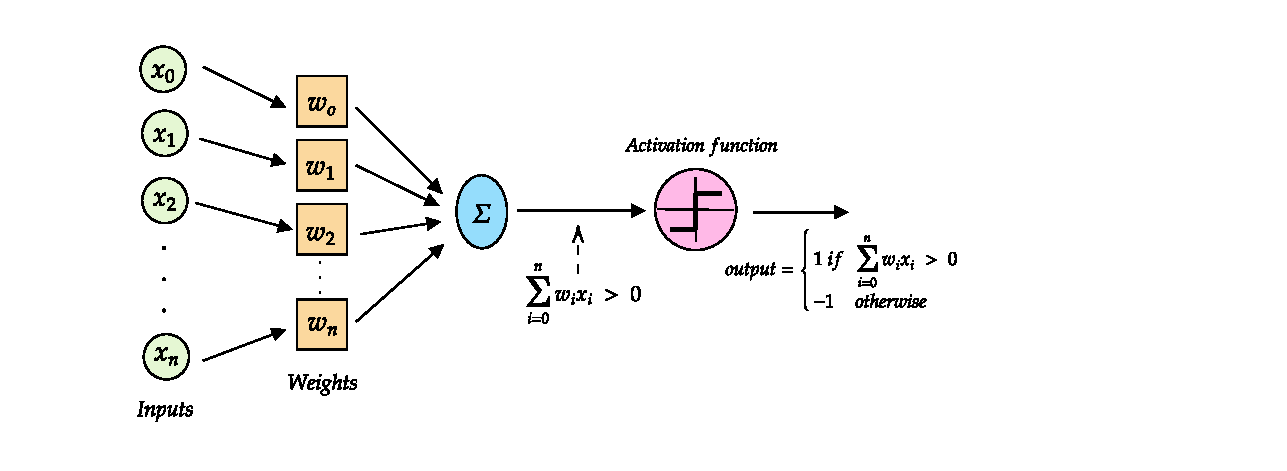
\includegraphics[width=0.8\linewidth]{Images/5.SPANet/one neuron.pdf}
    \caption{Fundamental unit of a Neural Network. The inputs are associated with a weight, that the network learns to optimize in the training. The weighted sum of the inputs and the weights constitutes the input to the activation function. The outcome of the activation function gives the prediction by the network.}
    \label{fig: neuron}
\end{figure}

Figure \ref{fig: neuron} shows the basic structure of the perceptron. Each input $x^i$ is characterized by a weight $w^i$ that connects the inputs to the artificial neuron. The weighted average is computed and is used as input of the activation function $\sigma$. The output of the network $\hat{y}$ is then given by:
\begin{equation}
    \hat{y}=\sigma\bigg(\sum_{i=0}^n w^i x^i\bigg)
    \label{eq: output network}
\end{equation}

\subsubsection{Activation functions}
The activation function transforms the weighted average input from the node into the output as shown Eq.(\ref{eq: output network}) \cite{ACTIVATION_FUNCTION}. Figure \ref{fig: activation function} shows some of the most commonly used activation functions:

\begin{itemize}
    \item The sigmoid function defined as:
    \begin{equation}
        \sigma(x)=\frac{1}{1+e^{-x}}
    \end{equation}
    \item The Rectified Linear Unit (ReLU) function defined as:
    \begin{equation}
        \sigma(x)=max(0,x)
    \end{equation}
    \item The softmax function defined for the i-th element as:
    \begin{equation}
        \sigma(x_i)=\frac{e^{x_i}}{\sum_{i=1}^n e^{x_i}}
    \label{eq: activation function}
        \end{equation}
\end{itemize}

\begin{figure}[hbt]
    \centering
    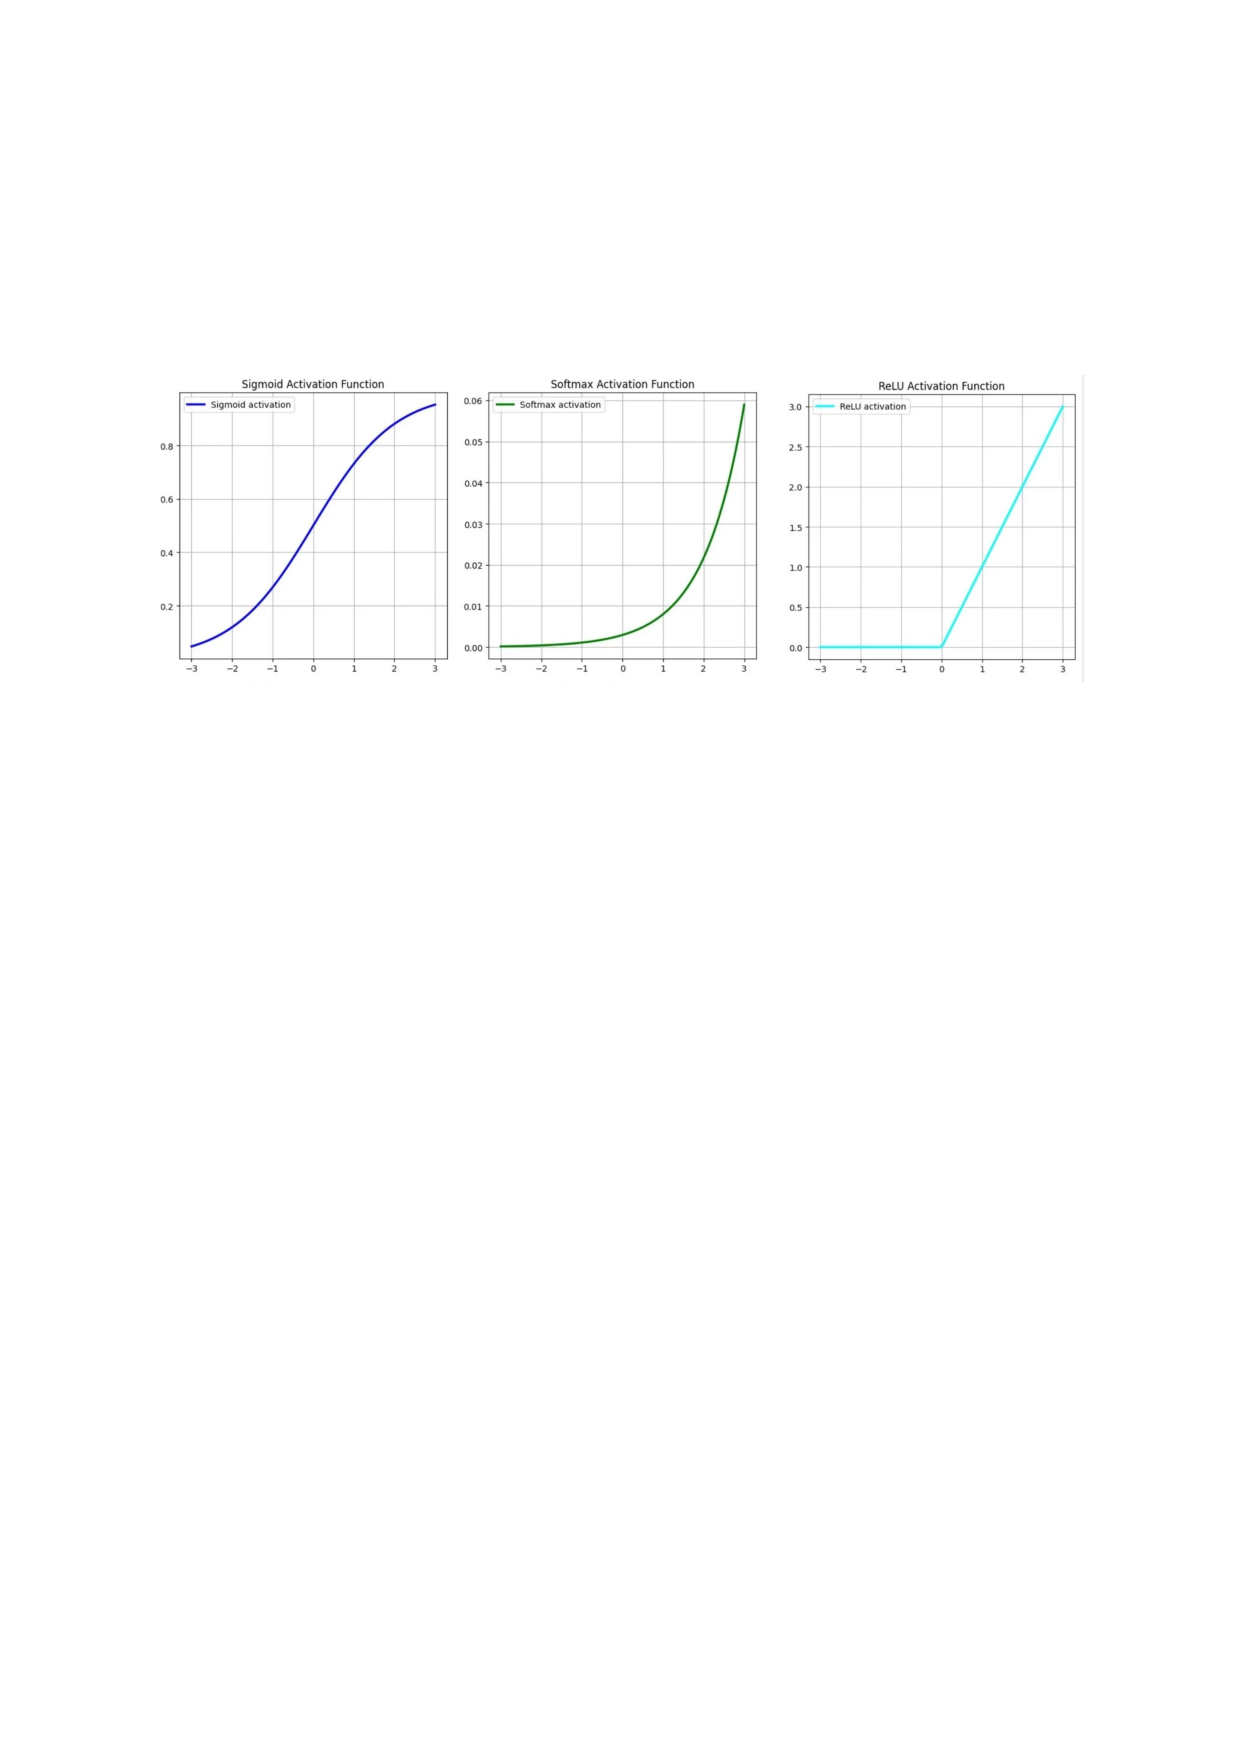
\includegraphics[width=0.7\linewidth]{Images/5.SPANet/Activation function 2.pdf}
    \caption{Examples of commonly used activation functions in machine learning. These plots show the sigmoid, softmax and ReLu functions \cite{figactivf}.}
    \label{fig: activation function}
\end{figure}

\subsubsection{Loss function}

The prediction of the neuron is computed using Eq.(\ref{eq: output network}) and the error of this output is computed using the loss function. The loss function $L$  allows to evaluate how good the prediction of the network is \cite{loss_function}. To optimize the model efficiently, depending on the task (classification, regression, etc.) different loss functions are required. Here two of the most commonly used loss functions are presented:

\begin{itemize}
    \item Mean squared error (MSE): This loss function is typically used in regression problems. It is computed by taking the squared difference between the predictions by the network and the truth target values. This squared difference is averaged across the dataset.
    \item Binary cross-entropy function: This loss function is typically used for binary classification tasks. This allows the measurement of the difference between the prediction $\hat{y}$ and the true binary label $y$. It can be computed as follows:
    \begin{equation}
        L(\hat{y},y)=-(y \text{log}(\hat{y}) + (1-y)  \text{log}(1-\hat{y}))    \end{equation}
\end{itemize} 

\subsubsection{Training of the perceptron}

Given a set of inputs $\{x\}_i$, the neural network aims to find the best set of weights $\{w\}_i$ that approximates the activation function $\sigma(x,w)=\hat{y}$, such that the predictions $\hat{y}$ are close to the target values $y$. The optimal values of the weights are found by training the network. For simplicity, the training of the perceptron, with only 1 neuron is presented, but this can be generalized to k neurons. The training of the perceptron consists of three steps:

\begin{itemize}
    \item[1.] Random initialization of the weights $w$
    \item[2.] Forward propagation: The prediction $\hat{y}$ is computed using Eq.(\ref{eq: output network}) and the loss function is also computed to obtain the error of the prediction.
    \item[3.] Backward propagation: The gradient of the loss function is computed, i.e. the partial derivatives of the loss function with respect to the weights $w$. The value of the weights is then updated by using the gradient and introducing the learning rate $\lambda$:
    \begin{equation}
        w_{new}=w-\lambda \nabla_w L
    \end{equation}
    Finally, the prediction $\hat{y}$ is computed again using the updated weights.
\end{itemize}

In the backward propagation, the learning rate $\lambda$ is introduced. It determines the step size taken into the gradient direction \cite{Learning_rate}, therefore a good choice for this parameter is essential. 
%As it is observed in Figure \textbf{bla}, 
If the learning rate is too small the gradient descent will be too slow, on the contrary, if it is too large it is possible to never reach the minimum, which can lead to divergent behaviors.

As mentioned, in this Section the training of neural networks is exemplified by using the perceptron which has only one neuron. Nevertheless, neural networks refer to models having multiple layers and multiple neurons per layer.  The first layer is the input layer which is responsible for transforming the raw input data into a format the network can understand and pass it to the hidden layers \cite{layers}.  These process the information and are located between the input and output layers. Finally, the output layer computes the final prediction. Even if the number of neurons and layers is increased, the principles of the training remain the same. In the forward propagation, the inputs are given to the network to compute an output and in the backward propagation, the gradients of the weights are computed in order to update the weights. This forward and backward propagation is repeated for multiple epochs until the loss function is minimized. The epochs refer to the passage of the entire dataset training through the learning algorithm \cite{epoch_batch}. The epochs are divided into batches. When dividing the epochs in batches, the forward propagation is computed per event, then the total loss is computed for one batch as the sum of the loss functions per event and finally, the backward propagation can be applied to this total loss per batch.

\subsubsection{Datasets used in ML}

The datasets in the training need to be large enough to represent the target distribution used. Typically this dataset is split as follows:
\begin{itemize}
    \item Train set: used for the forward and backward propagation
    \item Validation set: used during the training to check the training on a set that is statistically independent than the training set. After each batch, the model is evaluated on this dataset and therefore the performance can be evaluated.
    \item Test set: once the full training is complete this dataset is used to test the trained model on an independent set.
\end{itemize}

The validation step during the training allows for the prevention of under or overtraining. The training loss is high when underfitting since the predicted and true target values are too different. On the other hand, overfitting occurs when a model is learning the statistical fluctuation of the training data. Therefore, when overfitting occurs the overall loss is small but the validation loss, i.e. the loss of the model applied to the validation set, increases. 

%Figure \textbf{bla} shows an example of underfitting, correctly fitting, and overfitting.


The validation accuracy is defined as the percentage of the number of correctly predicted events over the total number of events. When the validation accuracy as a function of the training epochs reaches a stable plateau the training needs to be stopped to avoid overfitting. The validation accuracy and loss give complementary information. If the validation accuracy is high, the validation loss will be small. Figure \ref{fig: validation} shows an example of trainings done with SPANet (discussed in Section \ref{subsection: SPANet}) presented in Section \ref{section: improving}, where the validation accuracy tends to one, thus is high while the validation loss tends to zero.

\begin{figure}[h!]
    \centering
    \begin{subfigure}[b]{0.45\textwidth}
        \centering
        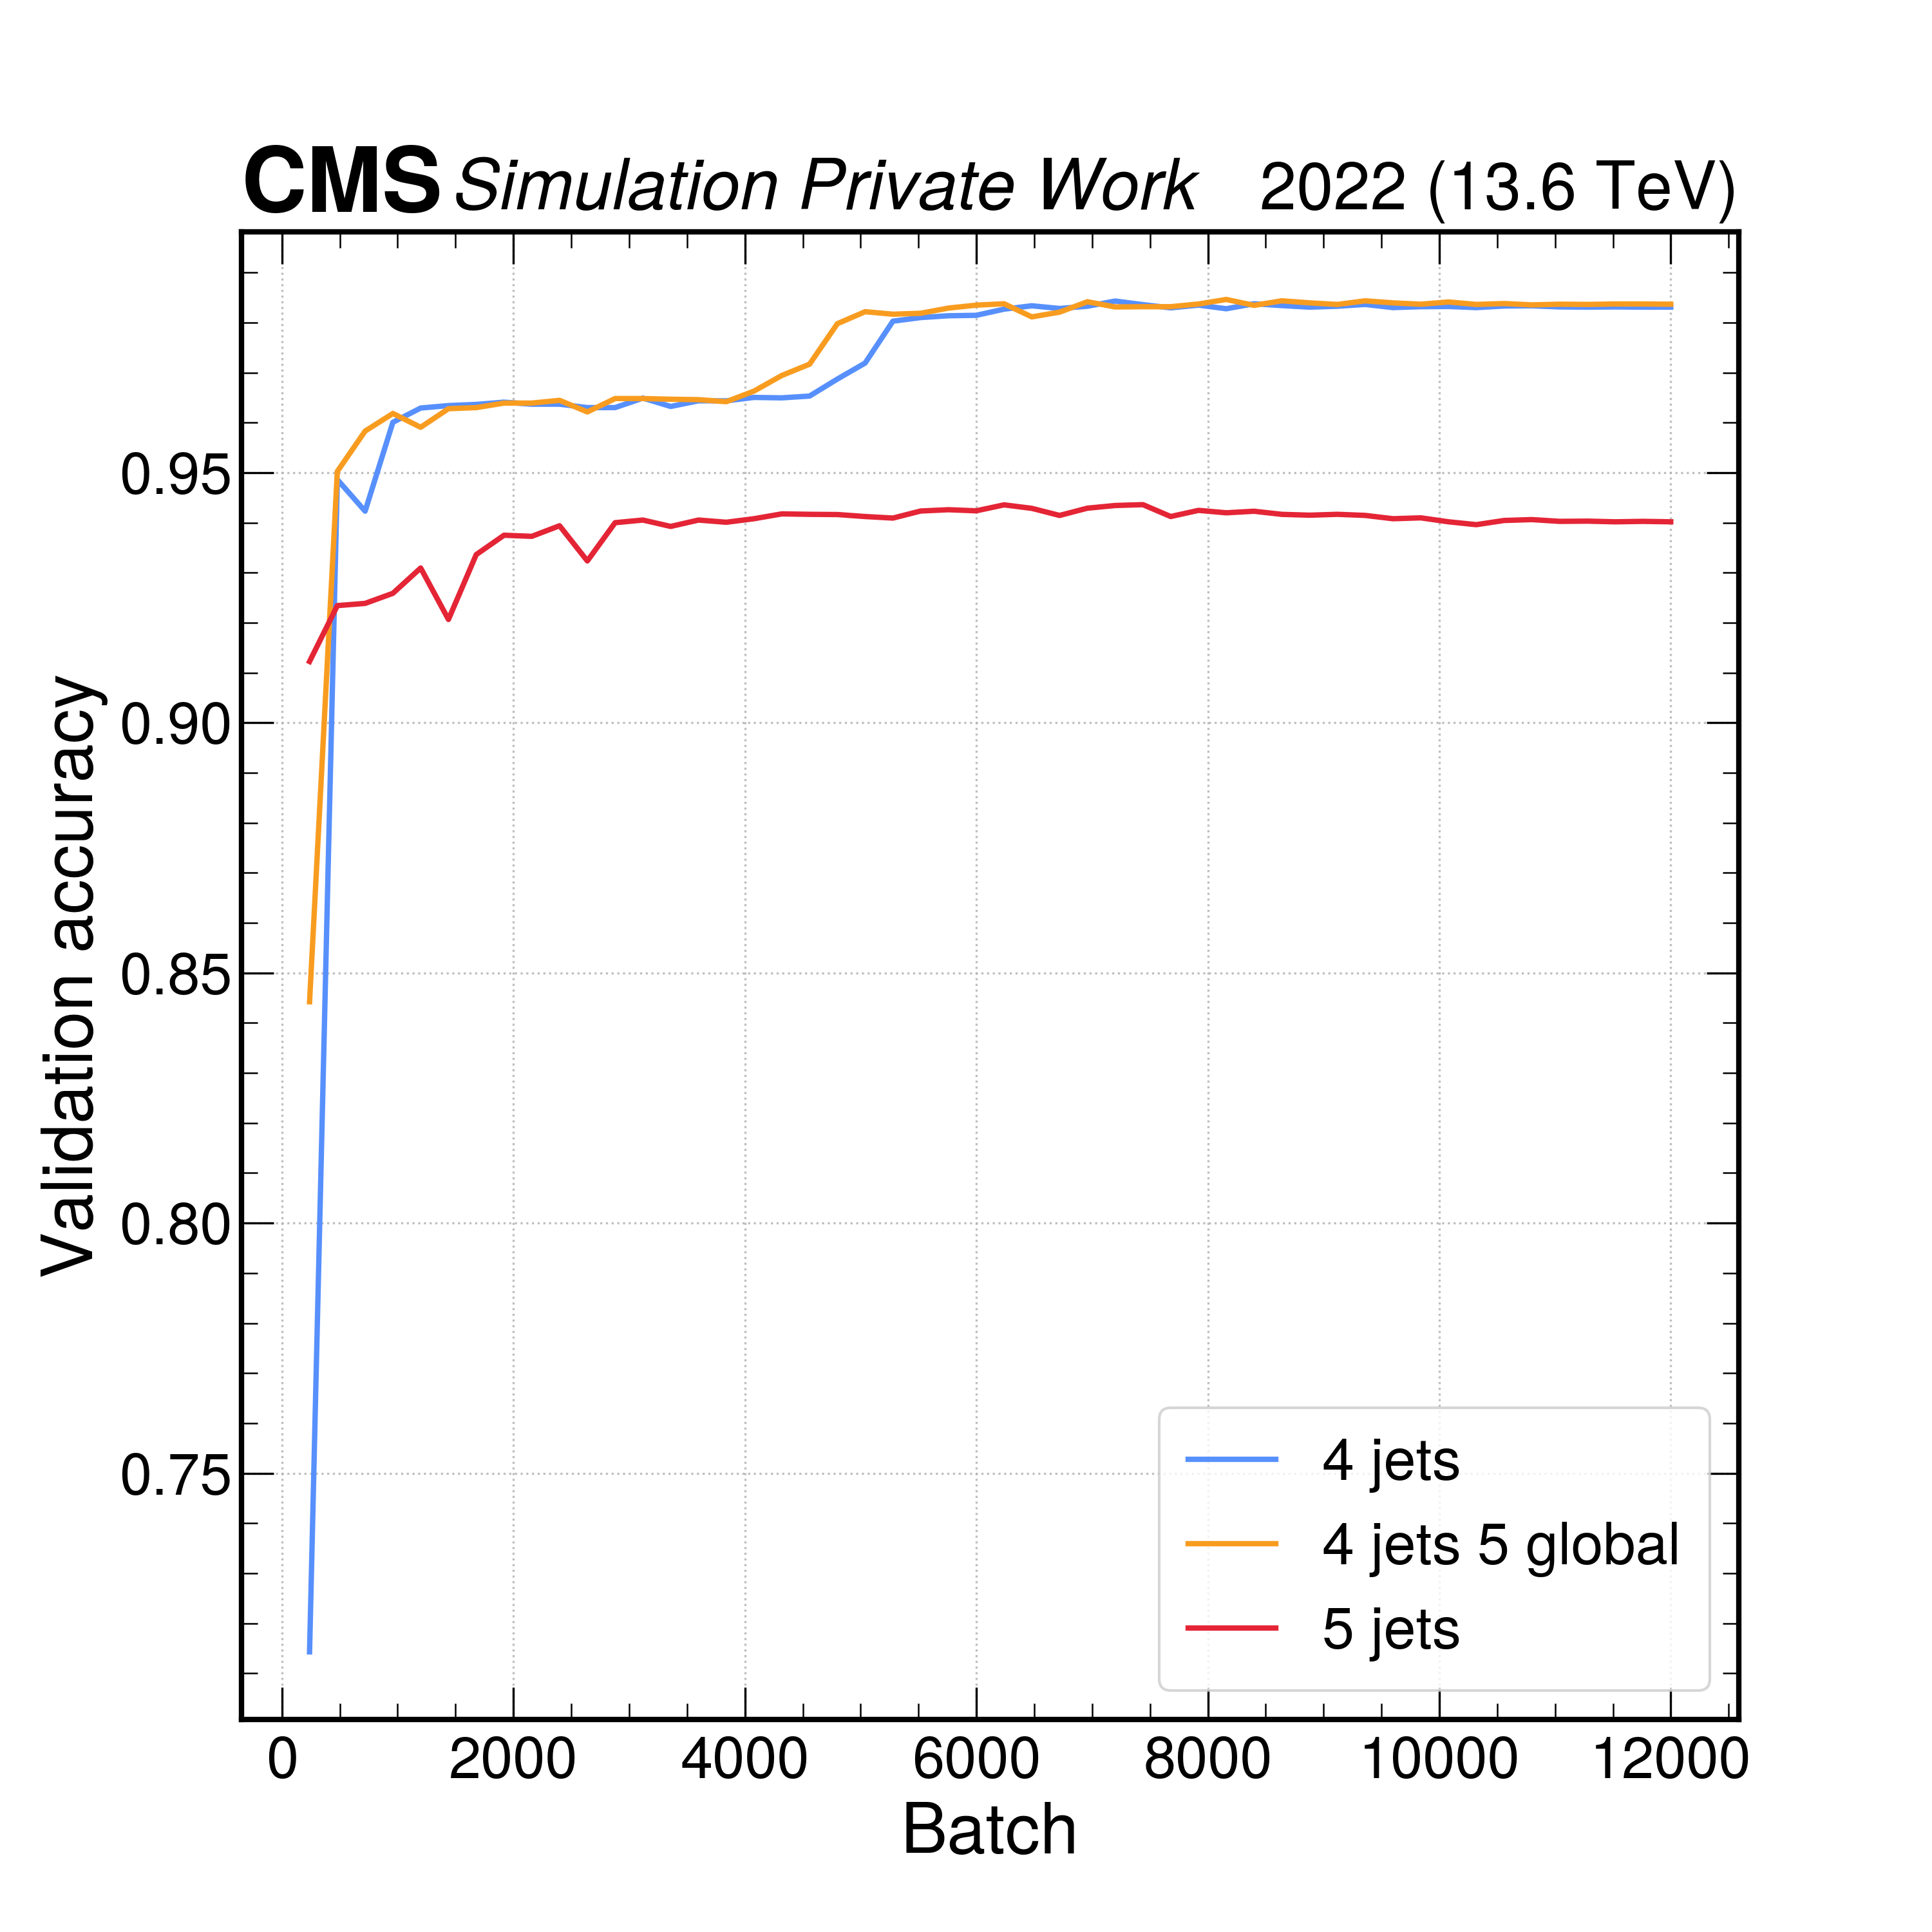
\includegraphics[width=\textwidth]{Images/5.SPANet/comp_4_4j5_5.png}
        % \caption{\pt of the leading Higgs.}
        % \label{fig: pt h1}
    \end{subfigure}
    \hfill
    \begin{subfigure}[b]{0.45\textwidth}
        \centering
        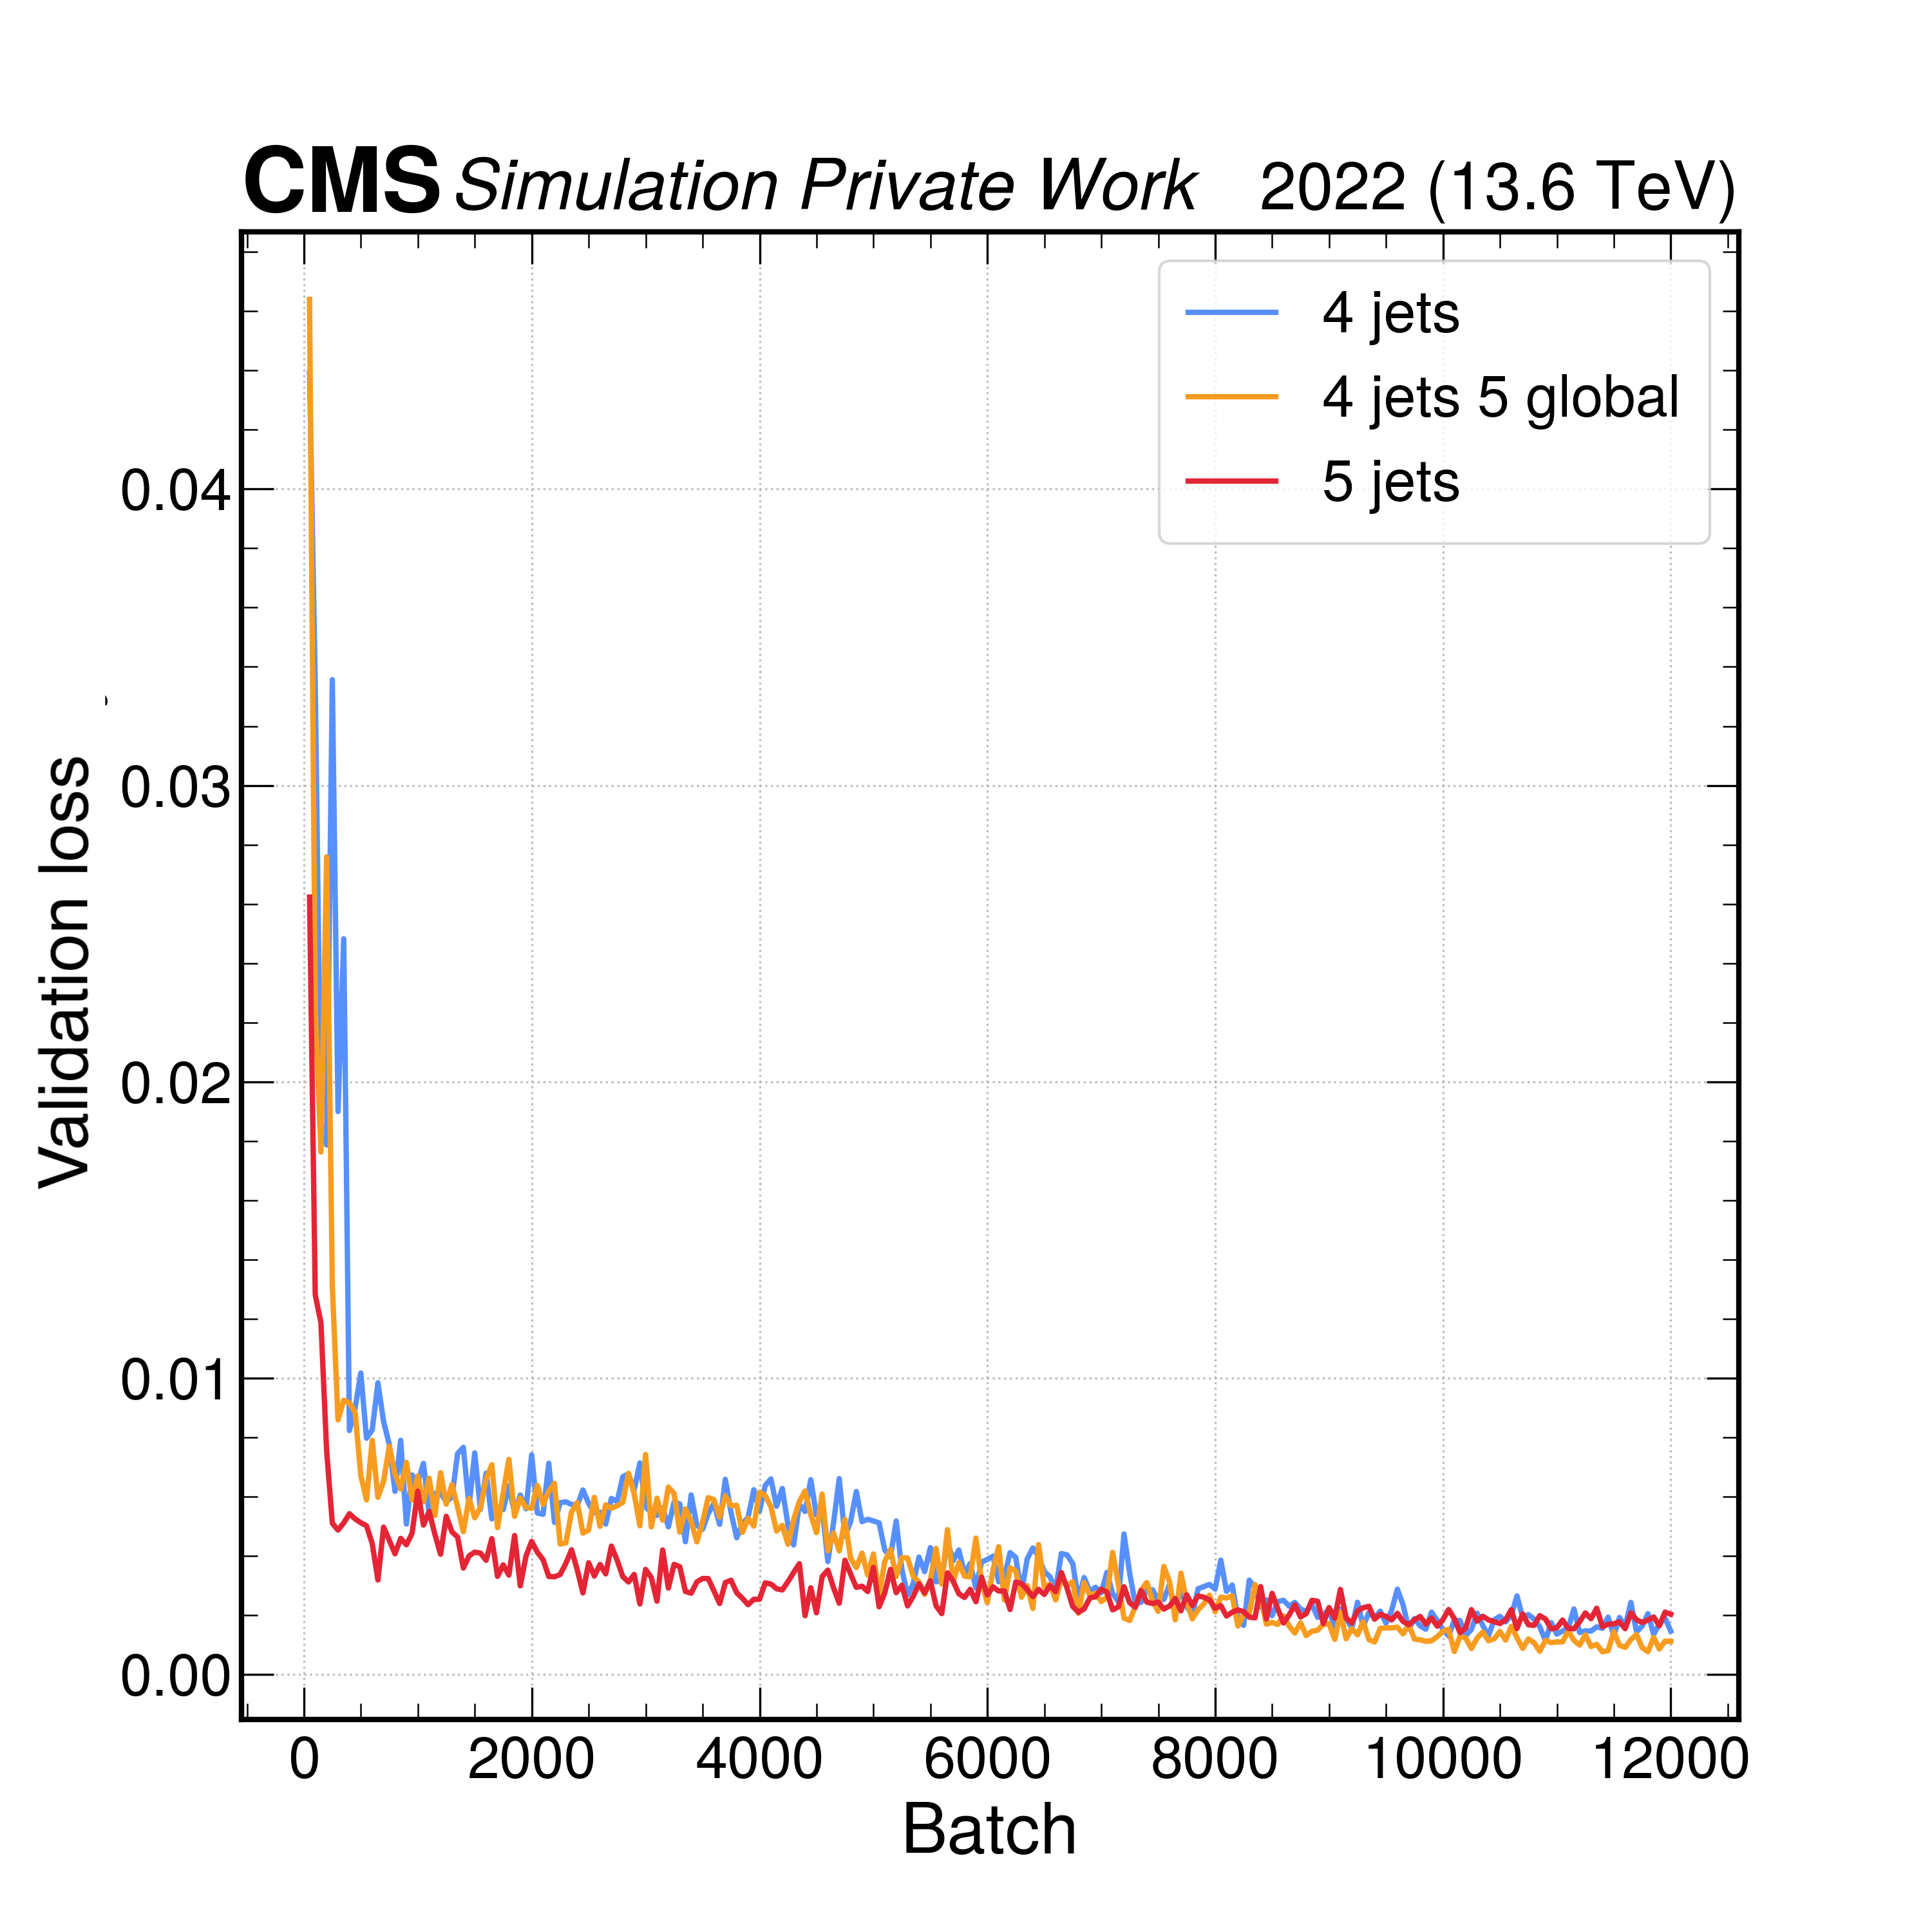
\includegraphics[width=\textwidth]{Images/5.SPANet/validation_loss.png}
        % \caption{\pt of the subleading Higgs.}
        % \label{fig: pt h2}
    \end{subfigure}
    \caption{Example of the validation loss and the validation accuracy plots of trainings done with SPANet (Section \ref{subsection: SPANet}) presented in Section \ref{section: improving}.}
    \label{fig: validation}
\end{figure}

\subsubsection{Transformers} \label{subsection: Attention based transformers}

Transformers are a specific type of neural network originally introduced in \cite{attentiontransformer} to translate one language to another. Figure \ref{fig: transformer architecture} shows the simplified architecture of a transformer. Such neural networks are capable of focusing on important words in a sentence, understanding the context and how words are related to each other as well as predicting the next words that can come in the sentence. As observed in Figure \ref{fig: transformer architecture}, the transformer architecture consists of two main components, the encoder and the decoder. The inputs, in the case of \cite{attentiontransformer}, are sentences made of strings given to the network. Nevertheless, for the network to process this information these words need to be converted into numerical vectors, which is done in the input embedding layer. These inputs are then forwarded to the encoder that processes these input sequences in the self-attention and feed-forward layers. The self-attention layer is a crucial component in the architecture as it allows to recognize the relationships and dependencies between objects, in this example the words in a sequence. More information on this can be found in \cite{attentiontransformer}. The feed-forward layer is a neural network layer whose inputs are the self-attention layer outputs. This neural network allows to extract meaningful information from the input sequences that are useful to determine the final output. This process can be repeated several times in the encoder. Finally, the output of the encoder is used as input to the decoder. The latter will generate the output of the network, which in the example treated in this Section can be either a translation or a text continuation. The output is passed through the activation function softmax function (see Eq. (\ref{eq: activation function})) that allows to map the outputs of the decoder into probability distributions.
\begin{figure}[hbt]
    \centering
    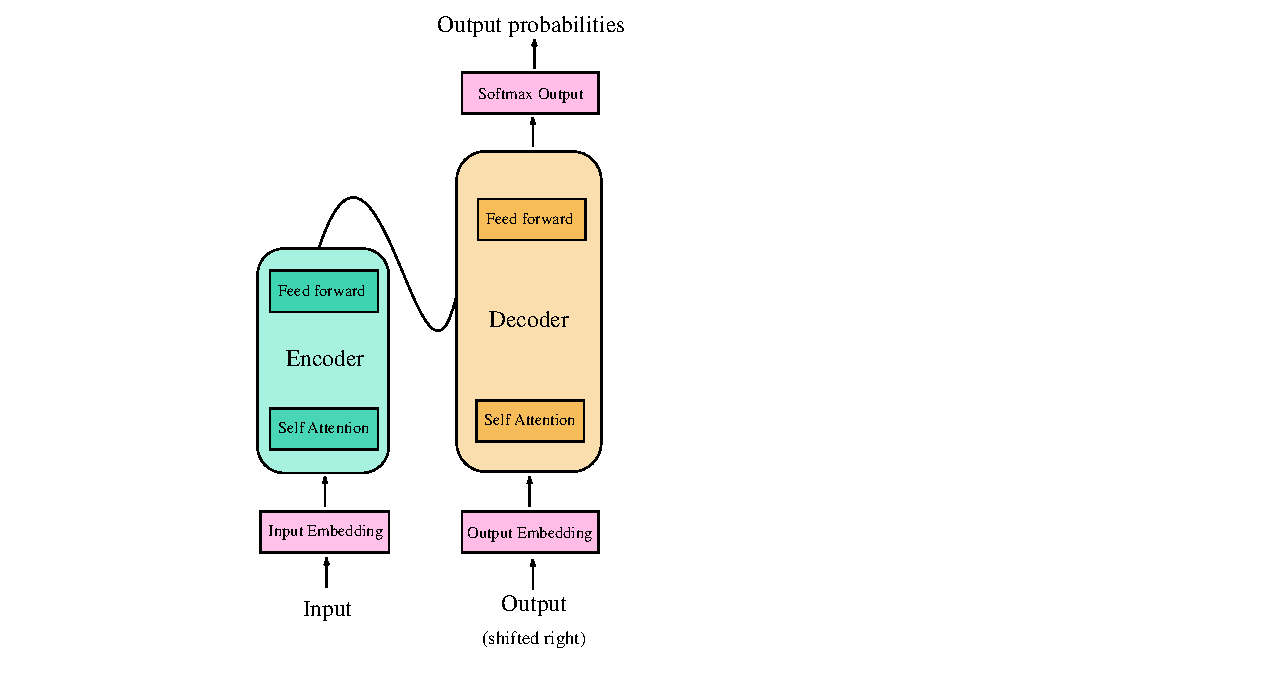
\includegraphics[width=0.4\linewidth]{Images/5.SPANet/transformer architecturepdf.pdf}
    \caption{Simplified transformer architecture. Two main components constitute a transformer: the encoder followed by the decoder.}
    \label{fig: transformer architecture}
\end{figure}


\subsection{Symmetry Preserving Attention Network: SPANet} \label{subsection: SPANet}
Attention-based deep learning methods, like transformers (described in Section \ref{subsection: Attention based transformers}), have achieved excellent performances in different problems so far. Nevertheless, they do not have built-in mechanisms to take into account the internal physical symmetries in assignment problems between sets, for instance in this case sets of jets. Therefore in \cite{SPANet} a new method for constructing symmetry-preserving attention networks (SPANet) is presented. As mentioned in Section \ref{subsection: run2 pairing}, in the HH $\to$ 4b analysis two symmetries are present in the pairing of the reconstructed jets to the generator-level quarks. On the one hand, the so-called jet symmetries: quark and anti-quark cannot be experimentally distinguished, therefore their labels can be swapped. On the other hand, there are particle symmetries, i.e. the symmetry of the exchange of the reconstructed Higgs candidate. As long as the jets are correctly paired to the generator-level quarks, it is not important whether they decay from H1 and H2. As will be shown in Section \ref{STA}, accounting for the jet and particle symmetries in the HH $\to$ 4b final state for the jet paring task significantly reduces the number of possible jet assignments

\begin{figure}[hbt]
    \centering
    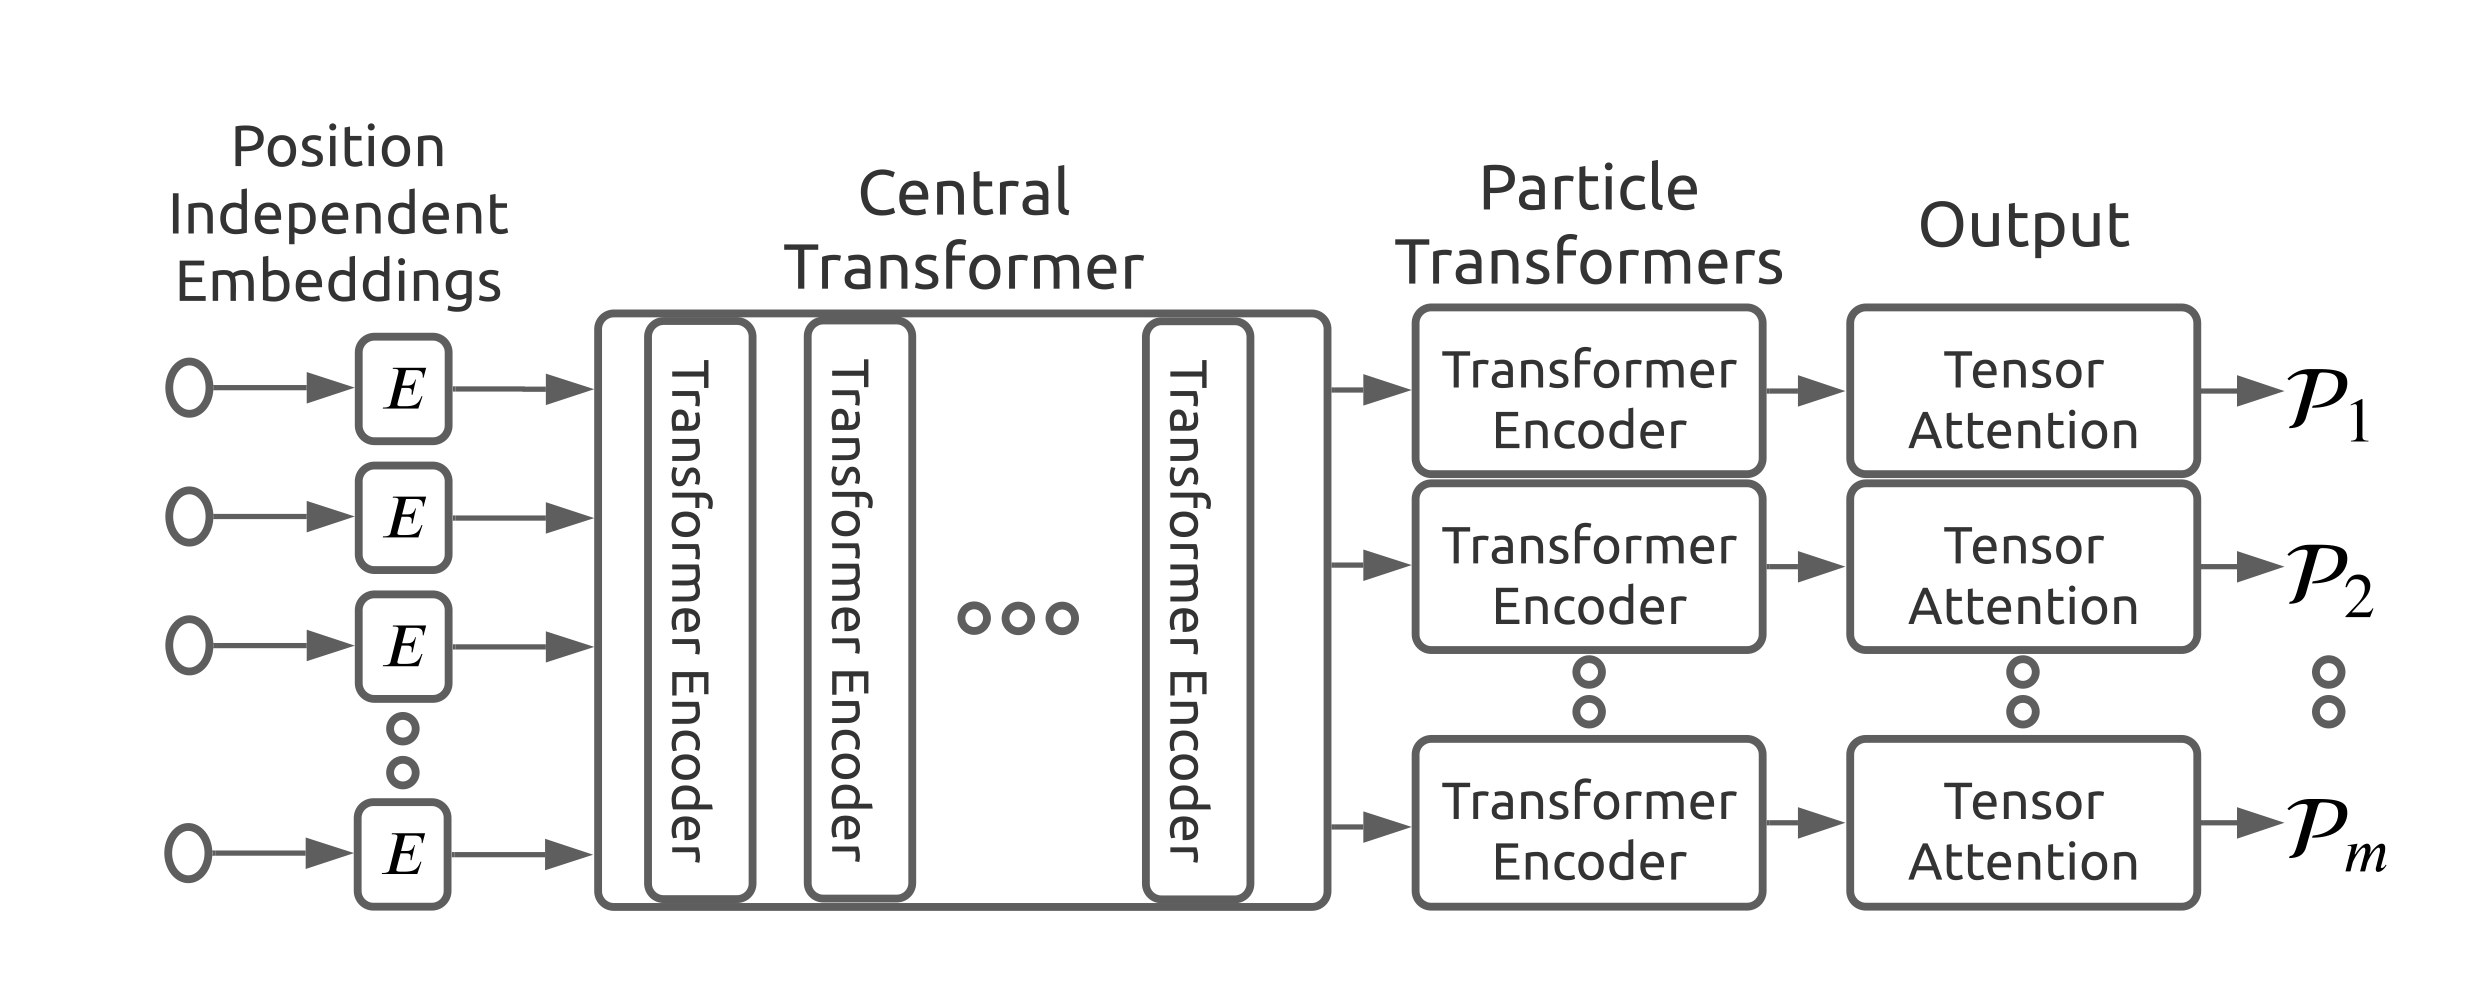
\includegraphics[width=0.7\linewidth]{Images/5.SPANet/SPANet structure.jpeg}
    \caption{High-level structure of SPANet from \cite{SPANet}. The inputs are passed to the transformer encoders which are followed by the tensor attention layer that produces the final output.}
    \label{fig : SPANet}
\end{figure}

Figure \ref{fig : SPANet} shows the high-level structure of SPANet. The network consists of an input layer, that takes as raw inputs the jets and produces jet embeddings, i.e. representations for each jet that will be fed to the central transformers. After the central encoder, additional transformer encoders for each particle, these being $H_1$ and $H_2$ in the scope of the HH $\to$ 4b analysis, are added to the network. The transformer encoders employ the multi-head self-attention \cite{attentiontransformer} but instead of positional text embeddings, position-independent jet embeddings are used as inputs to preserve the permutation invariance. In the additional particle transformers, the jet-quark assignment is divided into sub-problems for each Higgs. Then, the jet-quark pairing is solved per sub-problem, using the attention tensors, and in the end, all the sub-problem solutions are combined into a final jet-quark assignment. Finally, a new tensor-attention layer that produces the jet-quark assignment distribution is introduced. The basics of this symmetric tensor attention (STA) are presented in the next Section. 

\subsubsection{Symmetric Tensor Attention} \label{STA}
 In the general case, the particles $p$ that are reconstructed ($H_1$, $H_2$) are associated with $k_p$ quarks ($b$ and $\Bar{b}$). The STA takes as inputs a set of transformer-encoded jets $X_p \in \mathbb{R}^{N\times D}$ where N is the number of jets and D is the size of the hidden representation. The output will be a rank-$k_p$ tensor $\mathcal{P}_p \in \mathbb{R}^{N\times N \times ... \times N} $, such that $\sum \mathcal{P}_p=1 $. This represents the matrix of probabilities of the jet pairings. For the HH to 4b analysis, $\mathcal{P}_p$ will be a rank 2 tensor, i.e. an $N \times N$ matrix in which each value corresponds to the jet pairing probability. As is illustrated in Section \ref{subsubsection: PD var}, $\mathcal{P}_p$ is obtained for $H_1$ and $H_2$. The diagonal terms must be 0 since a single jet cannot be paired with itself. In order to include the jet symmetry described in Section \ref{subsection: SPANet} per particle $p$, a partition-level permutation group $G_p \in S_{k_p}$ is introduced. This group acts on $k_p$-tuples and defines an equivalence relation between indistinguishable jet assignments that is satisfied when the indices of $\mathcal{P}_p$ commute with respect to $G_p$ \cite{SPANet}:

 \begin{equation}
     \forall \sigma \in G_p (j_1,j_2,...,j_{k_p}) \approx (j_{\sigma(1)},j_{\sigma(2)},...,j_{\sigma(k_p)}) \Leftrightarrow \mathcal{P}_p^{j_1,j_2,...,j_{k_p}} = \mathcal{P}_p^{j_{\sigma(1)},j_{\sigma(2)},...,j_{\sigma(k_p)}}
 \end{equation}

 % The index commutativity is enforced by using a general dot-product attention (cite) where the output's symmetries are mimicked by the mixing weights.
 
 In the context of the HH $\to$ 4b analysis, this will correspond to having $\mathcal{P}_p^{b_1,b_2}=\mathcal{P}_p^{b_2,b_1}$, leading to a symmetric matrix, where $b_1$ and $b_2$ are the quarks coming from the decay of one of the two Higgs bosons. To compute the probability output, the STA layer contains one rank-$k_p$ tensor parameter tensor $\Theta \in \mathbb{R}^{D\times D \times ... \times D}$. From this tensor, to take into account the jet symmetry, the STA starts by constructing the $G_p$ symmetric tensor $\mathcal{S}$ (Eq.(\ref{Eq: symmetry tensor})) as the sum overall $G_p$-equivalent indices of $\Theta$. This ensures the $G_p$ symmetry, which corresponds in our case to swapping $b_1$ and $b_2$ quarks coming from one Higgs. Once this symmetry tensor is constructed, a generalized dot-product attention \cite{SPANet} is computed between the jet embeddings $X_p$ and the symmetric tensor $\mathcal{S}$, As shown in Eq.(\ref{Eq: generalized dot product}), this operation allows the inclusion of the $G_p$ symmetry for the pairing.  Finally, a $k_p$-dimensional softmax normalizes the output tensor $\mathcal{O}$ and produces the distribution $\mathcal{P}_p$ with the pairing probabilities, as shown in Eq.(\ref{Eq: probability output}). 

 \begin{equation}
     \mathcal{S}^{i_1i_2...i_{k_p}}=\sum_{\sigma \in G_p} \Theta^{i_{\sigma(1)}i_{\sigma(2)}...i_{\sigma(k_p)}}
     \label{Eq: symmetry tensor}
 \end{equation}

 \begin{equation}
    \mathcal{O}^{j_1j_2...j_{k_p}}=X^{j_1}_{i_1}X^{j_2}_{i_2}...X^{j_{k_p}}{i_{k_p}}\mathcal{S}^{i_1i_2...i_{k_p}}
    \label{Eq: generalized dot product}
 \end{equation}

 \begin{equation}
     \mathcal{P}_p^{j_1j_2...j_{k_p}}=\frac{exp(\mathcal{O}^{j_1j_2...j_{k_p}})}{\sum_{j_1j_2...j_{k_p}}\mathcal{O}^{j_1j_2...j_{k_p}}}
     \label{Eq: probability output}
 \end{equation}
 \noindent In  Eq.(\ref{Eq: symmetry tensor}) and (\ref{Eq: generalized dot product}) the index $i$ corresponds to $i \in D$ and in Eq.(\ref{Eq: generalized dot product}) and (\ref{Eq: probability output}), index $j$ corresponds to $j \in N$. All these Equations \cite{SPANet} are expressed using Einstein summation notation.

 The STA produces a probability tensor $\mathcal{P}_p$ solution, for each particle's jet-quark assignment sub-problem, i.e. for each resonance ($H_1$ and $H_2$). The true sub-assignment target for each Higgs is given by a $\delta$-distribution containing one possible valid jet assignment $\{ \mathcal{T}_1, \mathcal{T}_2, ... \mathcal{T}_p \}$.  Therefore, the loss function in this context is the cross entropy (CE) for each particle $p$: $CE(\mathcal{P}_p, \mathcal{T}_p)$. To take the particle symmetry mentioned in Section \ref{subsection: SPANet} into account in the computation of the loss function the event-level symmetry $G_E \in S_p$ is introduced. The latter introduces an equivalence relation (Eq.(\ref{Eq: symmetry H1 H2})) over the resonances that allows to freely swap entire particles as long as each sub-problem remains correctly assigned.

 \begin{equation}
     \forall \sigma \in G_E (\mathcal{T}_1,\mathcal{T}_2,...,\mathcal{T}_{p}) \approx (\mathcal{T}_{\sigma(1)},\mathcal{T}_{\sigma(2)},...,j_{\sigma(p)}) 
     \label{Eq: symmetry H1 H2}
 \end{equation}

 \noindent The computation of the loss when introducing this symmetry becomes:

\begin{equation}
    \mathcal{L}_{min}= min_{\sigma \in G_E} \sum_{i=1}^m CE(\mathcal{P}_i, \mathcal{T}_\sigma(i))
\end{equation}

\noindent this expression allows to fit the minimum attainable loss within a given equivalence class, which in the HH $\to$ 4b case corresponds to swapping $H_1$ and $H_2$. Finally in the evaluation of the model on a test dataset, the highest probability between $\mathcal{P}_1$ and $\mathcal{P}_2$ is chosen, and the algorithm uses the other matrix to find the highest compatible probability and determine the two most likely pairings. This is explained in more detail in Section \ref{subsubsection: PD var}.

\subsubsection{Partial event reconstruction}

Although at generator-level all the quarks are expected to produce a jet, due for instance to the detector acceptance, this jet may not be reconstructed. The permutation methods described in Section \ref{STA} struggle with partial events as the predictions are typically only valid for full permutations. To take this into account an event-level mask $\mathcal{M}_p \in \{0,1\}$ is introduced. The computation of the loss becomes \cite{SPANet}:

\begin{equation}
    \mathcal{L}_{min}^{masked}=min_{\sigma \in G_E}\bigg( \sum_{i=1}^p \frac{\mathcal{M}_{\sigma(i)} CE(\mathcal{P}_i, \mathcal{T}_{\sigma(i)})}{CB(\mathcal{M}_{\sigma(1)}, \mathcal{M}_{\sigma(2)}, ..., \mathcal{M}_{\sigma(p)})}\bigg)
\end{equation}

\noindent where only the loss by reconstructed particles is included.  To avoid a bias of the network towards more common configurations, the effective class count for each partial combination $CB(\mathcal{M}_{\sigma(1)}, \mathcal{M}_{\sigma(2)}, ..., \mathcal{M}_{\sigma(p)})$ is introduced (see \cite{SPANet} for more details).

\subsubsection{SPANet hyperparameters}

The SPANet default hyperparameters are chosen using the Sherpa hyperparameter optimization library \cite{Sherpa} The AdamW optimizer \cite{AdamW} is used with $L_2$ regularisation on all parameter weights. The $L_2$ regularisation is a method to avoid overfitting as the complexity of the network increases. A regularisation term:

\begin{equation}
    \lambda \sum_i w^2_i
\end{equation}

\noindent is added to the loss function as a penalty term to be minimized. $w_i$ are the weights of the model, and $\lambda$ is a hyperparameter 
%(cite). 
If $\lambda$ is set to zero,  the standard loss function is retrieved, if $\lambda$ is too large, it can add too much weight to the computation of the loss leading to underfitting.


\subsubsection{SPANet implementation}

In practical terms, the implementation of SPANet can be found in  \url{https://github.com/Alexanders101/}. Figure \ref{fig: config} shows an example of a configuration file for the HH $\to$ 4b topology. The first section named \verb|INPUTS| lists the sequential inputs, in this case, the per-jet input variables, and the global inputs which have a single vector per event, in this case only the fifth jet present in the event. The global and sequential inputs will be described in more detail in Section \ref{section: improving}. In \verb|EVENTS|, the resonance particles of the HH $\to$ 4b topology are defined. Finally in \verb|PERMUTATIONS| we describe the particle and jet symmetries of the analysis (defined in Section \ref{subsection: SPANet}).

\begin{figure}[hbt]
    \centering
    \begin{verbatim}
    INPUTS:
        SEQUENTIAL:
            Jet:
              pt: log_normalize
              eta: normalize
              phi: normalize
              btag: none
        GLOBAL:
            FifthJet:
              pt: log_normalize
              eta: normalize
              phi: normalize
              btag: none

    EVENT:
      h1:
        - b1
        - b2
      h2:
        - b3
        - b4

    PERMUTATIONS:
        EVENT:
          - [ h1, h2 ]
        h1:
          - [ b1, b2 ]
        h2:
          - [ b3, b4 ]
\end{verbatim}
    \caption{Example of config file from the SPANet codebase for the HH $\to$ 4b topology shown in Figure \ref{fig: topology}.}
    \label{fig: config}
\end{figure}

In Sections \ref{section: improving} and \ref{section: s/b classification} the results for the pairing and classification problems using SPANet are discussed. 